\section{Representação Intermediária de Código}\label{sec:IR}

Um compilador é um programa responsável por traduzir um código escrito em uma linguagem de programação para outra, geralmente do código-fonte para código de máquina, permitindo assim a execução do programa.
Durante esse processo, é fundamental que o mínimo de informações seja perdido, uma vez que a semântica original deve ser preservada no processo de tradução.
Uma abordagem comum utilizada para manter a integridade semântica e possibilitar otimizações, são as representações intermediárias (IR, do inglês \textit{intermediate representation})~\cite{cooper2014}.

Compiladores modernos, amplamente utilizados na indústria, empregam mais de uma IR para tirar proveito das vantagens de cada uma, uma vez que essas representações são projetadas para diferentes objetivos, como otimizações específicas.
As IRs podem ser classificadas de acordo com o nível de abstração e são comumente aplicados em sequência.
Representações com um nível maior de abstração são usadas próximas ao código-fonte, enquanto aquelas de nível mais baixo estão mais próximas do código de máquina~\cite{aho2008compilers}, como ilustrado na Figura~\ref{fig:abstraction-level-irs}.

\begin{figure}
  \centering
  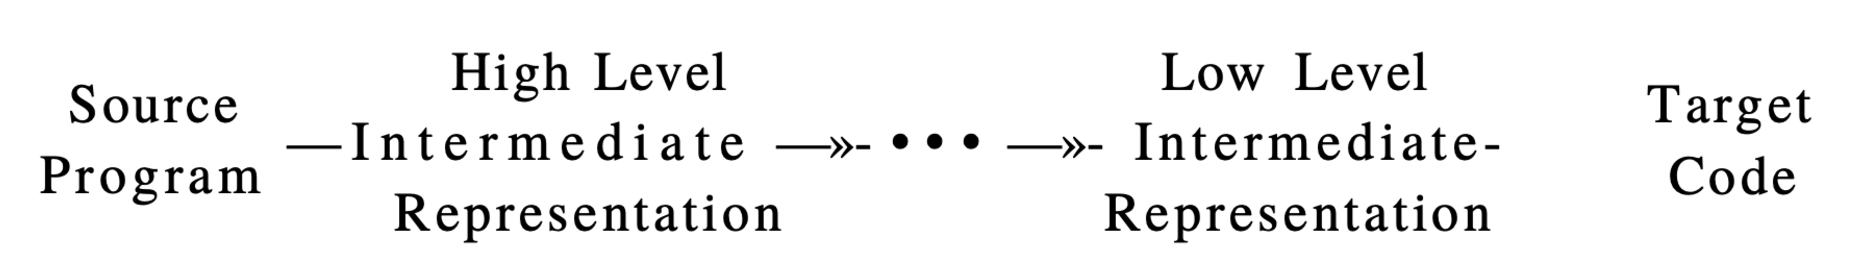
\includegraphics[width=.7\textwidth]{Imagens/abstraction-level-irs.eps}
  \caption{Sequência de representações intermediárias}\label{fig:abstraction-level-irs}
  \small{Fonte:~\cite{aho2008compilers}}
\end{figure}

Uma das principais informações que deve ser preservada em uma IR, é o fluxo de controle, isto é, a ordem em que as instruções do programa são executadas, como chamadas de função, \textit{loops} e condições.
Para garantir que o compilador mantenha a semântica correta do programa, o fluxo de controle deve ser repassado de alguma maneira durante o processo de tradução~\cite{cooper2014}.
Uma das maneiras disso ser feito explicitamente, é com o uso de continuações, que são funções que descrevem o próximo passo de uma computação em um ponto particular da execução do programa.

\subsection{CPS}\label{subsec:cps}

O estilo de passagem de continuações (CPS, do inglês \textit{continuation passing style}) é uma técnica de transformação de código que torna o fluxo de controle de um programa explícito, ao converter o estilo convencional de chamadas de função em chamadas que passam explicitamente o controle para a próxima etapa, conhecida como continuação (do inglês, \textit{continuation})~\cite{appel1992compiling}.
Em vez de retornar diretamente o resultado de uma função, o CPS transforma cada função para que, ao finalizar sua computação, ela invoque uma continuação, que representa o próximo passo a ser executado no programa.
Assim, toda chamada de função se torna uma chamada de cauda.

Uma chamada de cauda (do inglês \textit{tail call}) ocorre quando a última instrução executada em uma função é uma chamada a outra função, sem que restem computações adicionais a serem feitas após essa chamada~\cite{MUCHNICK1997}.
Isso permite que a função atual libere seu quadro de ativação, otimizando o uso de memória, já que o compilador não precisa manter o estado da função anterior na pilha.
Em constraste, uma chamada que não é de cauda ocorre quando ainda restam operações após a chamada, como somas ou multiplicações, o que exige que o quadro de ativação da função atual permaneça na pilha até a conclusão dessas operações.

Na Figura~\ref{code:factorial_non_tail_call}, o exemplo da função fatorial demonstra uma chamada que não é de cauda, pois a chamada recursiva \texttt{factorial(n - 1)} não é a última operação a ser realizada.
A função precisa aguardar o retorno desta chamada para, então, multiplicar o resultado por \texttt{n}, o que impede a liberação do quadro de ativação até o término da multiplicação.

Em constrate, na Figura~\ref{code:factorial_tail_call} como exemplo, tem-se uma versão da função fatorial que utiliza chamada de cauda.
A função auxiliar \texttt{go} acumula o valor do cálculo diretamente em seu argumento \texttt{a}, e a chamada recursiva \texttt{go (n - 1) (a * n)} é a última instrução a ser executada.
Como não há operações pendentes após a chamada recursiva, o compilador pode otimizar a função, reutilizando o quadro de ativação da função \texttt{go} para a chamada subsequente, tornando o cálculo mais eficiente.

\begin{figure}
  \caption{Função fatorial em Haskell}
  \small{Fonte: o autor}
  \lstinputlisting[style=haskell, label=code:factorial_non_tail_call]{Code/factorial_non_tail_call.hs}
\end{figure}

\begin{figure}
  \caption{Função fatorial em Haskell com chamada de cauda}
  \small{Fonte: o autor}
  \lstinputlisting[style=haskell, label=code:factorial_tail_call]{Code/factorial_tail_call.hs}
\end{figure}

O cálculo lambda, definido por~\citeonline{church1932set}, é um sistema formal que serve como base para a maioria das linguagens funcionais.
Ele é capaz de representar qualquer computação utilizando abstrações e aplicações através de reduções.
Sua sintaxe consiste em três regras simples que definem os elementos principais do sistema: variável, abstração e aplicação, conforme apresentados a seguir:

\begin{equation}\label{eq:lambda-calculus}
  e ::= x \mid \lambda x. e \mid e e
\end{equation}

A partir dessa sintaxe, um termo $e$ pode possuir apenas uma das três formas.
A primeira forma refere-se às variáveis, que representam identificadores no sistema.
A segunda forma, chamada de abstração, define uma função lambda: uma função que associa o identificador $x$ a um termo $e$, seu corpo, com $x$ vinculado ao termo $e$.
Finalmente, a aplicação ocorre quando um termo $e$ é aplicado a outro $e$, representando a chamada de uma função.

No cálculo lambda, as variáveis podem ser classificadas como livres ou ligadas, dependendo de seu contexto em um termo.
Variáveis são consideradas livres quando não estão associadas a uma abstração de função.
Por exemplo, no termo $\lambda x. y$, a variável $y$ é livre, pois não está ligada a nenhum parâmetro introduzido.
Em contraste, no termo $(\lambda x. x) y$, a variável $x$ está ligada dentro do corpo da abstração, enquanto $y$ permanece livre.
Um termo sem variáveis livres é denominado fechado ou combinador; por exemplo, $\lambda x. \lambda y. x y$ é um combinador, pois todas as variáveis estão ligadas às suas respectivas abstrações.

Para avaliar expressões no cálculo lambda, usamos três tipos de redução: $\alpha$, $\beta$ e $\eta$, que seguem as seguintes definições:

\begin{description}
  \item[$\alpha$-redução:] Renomeação de variáveis ligadas.
    \begin{align}
      \lambda x . e[x] & \rightarrow \lambda y . e[y]\label{eq:alpha-reduction}
    \end{align}

  \item[$\beta$-redução:] Aplicação de função.
    \begin{align}
      (\lambda x . e_1) e_2 & \rightarrow e_1 [e_2 / x]\label{eq:beta-reduction}
    \end{align}

  \item[$\eta$-redução:] Expansão de função.
    \begin{align}
      \lambda x . (e \, x) & \rightarrow e \quad \text{se } x \text{ não ocorre livre em } e\label{eq:eta-reduction}
    \end{align}
\end{description}

As reduções são responsáveis pela semântica operacional do cálculo lambda.
A $\alpha$-redução permite a renomeação de variáveis ligadas, enquanto a $\beta$-redução descreve a aplicação de funções, substituindo o parâmetro da função por um valor passado como argumento.
Por fim, a $\eta$-redução lida com a simplificação de funções quando elas aplicam diretamente seu argumento.

A transformação para CPS se baseia nessa estrutura formal.
No cálculo lambda tradicional, o fluxo de execução é implícito: as funções são aplicadas e seus resultados são retornados automaticamente.
No entanto, no CPS, o fluxo de controle é explicitamente representado como uma série de chamadas a funções.
Cada função, em vez de retornar diretamente um valor, recebe um argumento extra, a continuação, que indica o próximo passo da computação.

Por exemplo, a expressão $\lambda x. x + 1$ no cálculo lambda tradicional retornaria o valor $x + 1$. Ao transformar essa expressão para CPS, ela se torna $\lambda x. \lambda k. k (x + 1)$.

Aqui, $k$ é a continuação que processa o resultado $x + 1$.
Essa técnica é especialmente poderosa no contexto de compiladores, uma vez que facilita várias formas de otimizações e análises, como eliminação de recursividade em cauda (TCO, do inglês \textit{tail-call optimization}), expansão \textit{inline}, representação de \textit{closures}, alocação de registradores, entre outras~\cite{appel1992compiling}.
Ao transformar o código para CPS, todo o fluxo de execução do programa é capturado como uma série de chamadas encadeadas de funções, sem depender de uma pilha de execução implícita.

O cálculo de continuações (do inglês, \textit{CPS-calculus}), conforme definido por~\citeonline{thielecke1997}, é um sistema formal que leva o CPS além de seu uso tradicional como uma técnica de transformação de código, tratando-o como um modelo computacional por si só.
Enquanto o CPS é utilizado como uma IR em compiladores, o cálculo de continuações oferece uma estrutura para raciocinar formalmente sobre computações onde o fluxo de controle é explicitamente representado.
Os termos do cálculo de continuações, chamados de comandos, são descritos pelas seguintes regras:

\begin{equation}
  M ::= x\langle \vec{x} \rangle \mid M\{x\langle \vec{x} \rangle = M\}
\end{equation}

% Explicar a sintaxe do cálculo de continuações
Aqui, $x\langle \vec{x} \rangle$ representa um salto (do inglês \textit{jump}), isto é, uma chamada para a continuação $x$ com os parâmetros $\vec{x}$, sendo essencialmente uma chamada direta para a continuação, enquanto $M\{x\langle \vec{x} \rangle = M\}$ representa um vínculo (do inglês \textit{binding}), onde o corpo $M$ está vinculado à continuação $x$ com os parâmetros $\vec{x}$, isto é, uma chamada intermediária que, ao ser chamada, executará o próximo passo da computação.
Vale ressaltar que \citeonline{APPEL1997} possuem uma sintaxe diferente para o cálculo de continuações, onde os termos são respectivamente representados como $k(\vec{x})$ e $\texttt{let }k(\vec{x}) = c \texttt{ in } b$.

A tradução para CPS converte um código escrito em estilo direto (onde o controle de fluxo é implícito) para o estilo de passagem de continuações~\cite{FLANAGAN1993}.
A principal ideia por trás dessa transformação é modificar as funções para que elas não retornem um valor diretamente, mas, em vez disso, passem o resultado para uma continuação.

\begin{figure}
  \caption{Função soma em Haskell em Estilo Direto}
  \small{Fonte: o autor}
  \lstinputlisting[style=haskell, label=code:add]{Code/add.hs}
\end{figure}

\begin{figure}
  \caption{Função soma em Haskell em CPS}
  \small{Fonte: o autor}
  \lstinputlisting[style=haskell, label=code:add_cps]{Code/add_cps.hs}
\end{figure}

Por exemplo, a Figura~\ref{code:add} apresenta um programa na linguagem Haskell que soma dois números no estilo direto, retornando o valor após realizar o cálculo.
Já a Figura~\ref{code:add_cps} mostra um programa equivalente em CPS\@.
Nesta versão, o controle de fluxo do programa é explícito, pois a função $k$ é chamada para processar o resultado da soma dos argumentos.

\begin{figure}
  \caption{Função fatorial em Haskell em Estilo Direto}
  \small{Fonte: o autor}
  \lstinputlisting[style=haskell, label=code:factorial]{Code/factorial.hs}
\end{figure}

\begin{figure}
  \caption{Função fatorial em Haskell em CPS}
  \small{Fonte: o autor}
  \lstinputlisting[style=haskell, label=code:factorial_cps]{Code/factorial_cps.hs}
\end{figure}

Para ilustrar melhor, a Figura~\ref{code:factorial} apresenta um programa em Haskell que calcula o fatorial no estilo direto, utilizando funções definidas para multiplicação e subtração.
Na Figura~\ref{code:factorial_cps}, um programa similar em CPS é definido, com as funções auxiliares também transformadas para CPS\@.
Na função \texttt{factorialCps} é possível notar duas funções lambda (continuações), \texttt{nMinus1} e \texttt{factNMinus1}.
A primeira continuação guarda o resultado da operação $n - 1$, enquanto a segunda recebe recursivamente o cálculo do fatorial de $n - 1$, multiplica por $n$ e finalmente passa o resultado para a continuação $k$.

Outro fato importante a se observado nos códigos apresentados é a tipagem das funções.
Na função de soma, definida na Figura~\ref{code:add}, a função tem tipo $Int \rightarrow Int \rightarrow Int$, ou seja, ela recebe dois inteiros e retorna um inteiro.
Já a função de soma em CPS, definido na Figura~\ref{code:add_cps}, possui o tipo $Int \rightarrow Int \rightarrow (Int \rightarrow r) \rightarrow r$. Isso significa que a função recebe dois inteiros e uma continuação, que é uma função de tipo $Int \rightarrow r$, onde \texttt{r} pode ser qualquer tipo, e retorna esse mesmo tipo \texttt{r}.

Essa transformação de tipo reflete a diferença fundamental entre o estilo direto e o CPS\@: em vez de retornar um valor diretamente, a função em CPS recebe uma continuação que especifica o próximo passo da computação.
O mesmo padrão pode ser observado nas funções para o cálculo do fatorial nas Figuras~\ref{code:factorial} e~\ref{code:factorial_cps}.
No estilo direto, a função \texttt{factorial} tem o tipo $Int \rightarrow Int$, enquanto na versão CPS, a função \texttt{factorialCps} tem o tipo $Int \rightarrow (Int \rightarrow r) \rightarrow r$.

Essa correspondência entre os tipos não é uma coincidência.
Como discutido por~\cite{TORRENS2019}, uma função em estilo direto com tipo $A \rightarrow B$ pode ser transformada em uma função em CPS com o tipo $A \rightarrow (B \rightarrow \perp) \rightarrow \perp$.
Aqui, $\perp$ representa o tipo dos valores que nunca retornam, uma característica associada ao estilo de passagem de continuações, onde as funções são compostas de forma a encadear continuações até que a execução termine de maneira explícita.

Este exemplo simples da função fatorial em CPS ilustra as dificuldades inerentes ao uso de continuações explícitas, como a verbosidade do código, complexidade de compreensão e a propensão a erros.
No entanto, apesar desses desafios, o CPS se mostra extremamente adequado para a aplicação de otimizações, sendo uma escolha eficiente para representações intermediárias, especialmente em cenários onde o desempenho é essencial.
